\documentclass[11pt]{article}

\usepackage[a4paper,margin=2.2cm]{geometry}
\usepackage{amsmath,amssymb}
\usepackage{graphicx}
\usepackage{subcaption}
\usepackage{booktabs}
\usepackage{siunitx}
\usepackage{xcolor}
\usepackage[hidelinks]{hyperref}
\usepackage{caption}
\captionsetup{font=small}

\newcommand{\eox}{\varepsilon_{\mathrm{ox}}}
\newcommand{\esi}{\varepsilon_{\mathrm{si}}}
\newcommand{\SD}{S_{D}}
\newcommand{\tox}{t_{\mathrm{ox}}}

\title{\vspace{-1.2cm}\textbf{Reproduction of Nakagawa, Yasuhara \& Baba
(ISPSD 1990)}\\[4pt]
\large ``New 500\,V Output Device Structures for Thin Silicon Layer on
Silicon Dioxide Film''\\ \normalsize Proc.\ ISPSD 1990, Tokyo, pp.~97--101}
\author{Independent derivation, simulation and figure-by-figure comparison}
\date{}

\begin{document}
\maketitle
\vspace{-0.8cm}

\begin{abstract}
\noindent A thin (\SI{20}{\micro\meter}) silicon layer on a buried silicon-dioxide
film (BOX) over a grounded substrate forms a lateral high-voltage diode. When the
silicon fully depletes, more than half of the applied \SI{500}{\volt} is forced
across the buried oxide, and a shallow $N$ donor layer (dose $\SD$) shields the
bulk silicon so avalanche is delayed. We derive the electrostatics, solve the
Poisson PDE in 1-D (drain symmetry axis) and 2-D (cross-section), add a Chynoweth
avalanche integral, and compare figure-by-figure with the paper. Figures~4, 5 and
6 (structure~B, the optimized device) reproduce quantitatively; Fig.~7
(structure~A) is a 2-D effect the vertical model captures only in trend.
\end{abstract}

\section*{Key results (model vs.\ paper)}
\begin{center}
\begin{tabular}{@{}lcc@{}}
\toprule
Quantity & Model & Paper \\
\midrule
Oxide voltage share ($\tox=\SI{3}{\micro\meter}$) & 54--60\,\% & $>50\,\%$ (Fig.~4) \\
Peak $BV$, $\tox=\SI{1}{\micro\meter}$ & \SI{401}{\volt} & $\sim\!\SI{380}{\volt}$ (Fig.~6) \\
Peak $BV$, $\tox=\SI{2}{\micro\meter}$ & \SI{479}{\volt} & $\sim\!\SI{480}{\volt}$ (Fig.~6) \\
Peak $BV$, $\tox=\SI{3}{\micro\meter}$ & \SI{565}{\volt} & $\sim\!\SI{580}{\volt}$ (Fig.~6) \\
RESURF optimum dose & $\sim\!10^{12}$ & $\sim\!10^{12}\ \mathrm{cm^{-2}}$ \\
Structure A needs thicker oxide & yes (2-D) & \SI{5}{\micro\meter} vs \SI{3}{\micro\meter} (Fig.~7) \\
\bottomrule
\end{tabular}
\end{center}

\section{Theory}

\subsection{The device and the key idea}
Under high reverse bias the thin silicon layer \emph{fully depletes}, and a large
fraction of the applied voltage is forced across the buried oxide --- so the
device blocks $\ge \SI{500}{\volt}$ with only \SI{20}{\micro\meter} of silicon.
The ionized (positive) donors of the shallow $N$ layer at the Si/BOX interface
``shield'' the bulk silicon: they let the field be large in the oxide while
keeping it low in the silicon, delaying avalanche.

\subsection{One-dimensional vertical model (drain symmetry axis $AA'$, structure B)}
Take $y$ downward, $y=0$ at the top of the silicon; the drain (top) is at the
applied voltage $V$ and the substrate (below the oxide) is grounded. Under full
depletion the charge density is $\rho = qN$ (donors positive) and Poisson's
equation is
\begin{equation}
\frac{d}{dy}\!\left(\varepsilon\,\frac{d\phi}{dy}\right) = -qN(y),
\qquad E = -\frac{d\phi}{dy}.
\end{equation}
The normal displacement $D=\varepsilon E$ is continuous across the Si/oxide
interface, so the field jumps \emph{up} into the oxide:
\begin{equation}
E_{\mathrm{ox}} = \frac{\esi}{\eox}\,E_{\mathrm{si}}
\approx \frac{11.7}{3.9}\,E_{\mathrm{si}} \approx 3\,E_{\mathrm{si}}.
\end{equation}
Modelling the shallow layer as an areal sheet $q\SD$, crossing it upward drops the
displacement by $q\SD$, so the field in the \emph{bulk} silicon is
\begin{equation}
\boxed{\,E_{\mathrm{si,bulk}} = \frac{D_{\mathrm{ox}} - q\SD}{\esi}\,}
\end{equation}
which \emph{decreases} as $\SD$ rises: the donor sheet shields the silicon (exactly
the Fig.~5 ordering $D>C>B>A$). Integrating $E$ over each region, the oxide share
$V_{\mathrm{ox}}/V$ grows with $\SD$ and $\tox$; at $\tox=\SI{3}{\micro\meter}$,
$\SD=\SI{1.5e12}{\per\square\centi\meter}$, $V=\SI{500}{\volt}$ the model gives
$V_{\mathrm{ox}}/V\approx0.60$ --- reproducing Fig.~4's ``more than half across
the oxide.''

\subsection{Avalanche breakdown and the RESURF optimum}
Avalanche occurs in the silicon (the oxide does not ionize). With the Chynoweth
ionization coefficient for silicon,
\begin{equation}
\alpha(E) = A\,e^{-B/E},\qquad
A = \SI{7.03e5}{\per\centi\meter},\quad
B = \SI{1.231e6}{\volt\per\centi\meter},
\end{equation}
breakdown occurs when the ionization integral along $AA'$ reaches unity:
\begin{equation}
I(V) = \int_{\mathrm{Si}} \alpha\big(|E(y)|\big)\,dy = 1
\;\;\Longrightarrow\;\; V = BV.
\end{equation}
Two competing effects set $BV(\SD)$: too little dose gives poor shielding and an
early avalanche; too much dose over-shields and the corner/oxide field grows. So
$BV(\SD)$ rises, peaks near the RESURF charge ($\sim\!\SI{1e12}{\per\square\centi\meter}$),
then falls --- the shape of Fig.~6. A thicker oxide shares more voltage and raises
the peak $BV$.

\subsection{Why structure A needs a thicker oxide (a 2-D effect)}
Structures A and B share the \emph{same} vertical stack, so a purely vertical
(1-D) or mirror-symmetric 2-D model cannot separate them. In structure~B the drain
sits directly over the oxide at the symmetry axis (most complete vertical
field-sharing, breakdown point \#1 under the drain); in structure~A the drain is
displaced and its critical point couples less completely to the grounded
substrate, so A needs a \SI{5}{\micro\meter} oxide where B needs
\SI{3}{\micro\meter}. The vertical model represents the favourable B-type sharing
and therefore over-predicts A.

\paragraph{Assumptions.}
$L_{\mathrm{si}}=\SI{20}{\micro\meter}$; $\tox=1$--\SI{5}{\micro\meter} (swept);
shallow-layer thickness $w_n=\SI{2}{\micro\meter}$ (``a few microns''); background
$n^-$ doping $N_{D0}=\SI{1e14}{\per\cubic\centi\meter}$ (not stated in the paper;
chosen to centre the Fig.~6 RESURF peak; standard for a \SI{500}{\volt}-class
\SI{20}{\micro\meter} drift layer); $\esi=11.7$, $\eox=3.9$.

\section{Figure-by-figure comparison}

\begin{figure}[h!]
\centering
\begin{subfigure}{0.44\textwidth}
\includegraphics[width=\linewidth]{../figs_paper/fig4_paper_crop.png}
\caption{Paper (original)}
\end{subfigure}\hfill
\begin{subfigure}{0.52\textwidth}
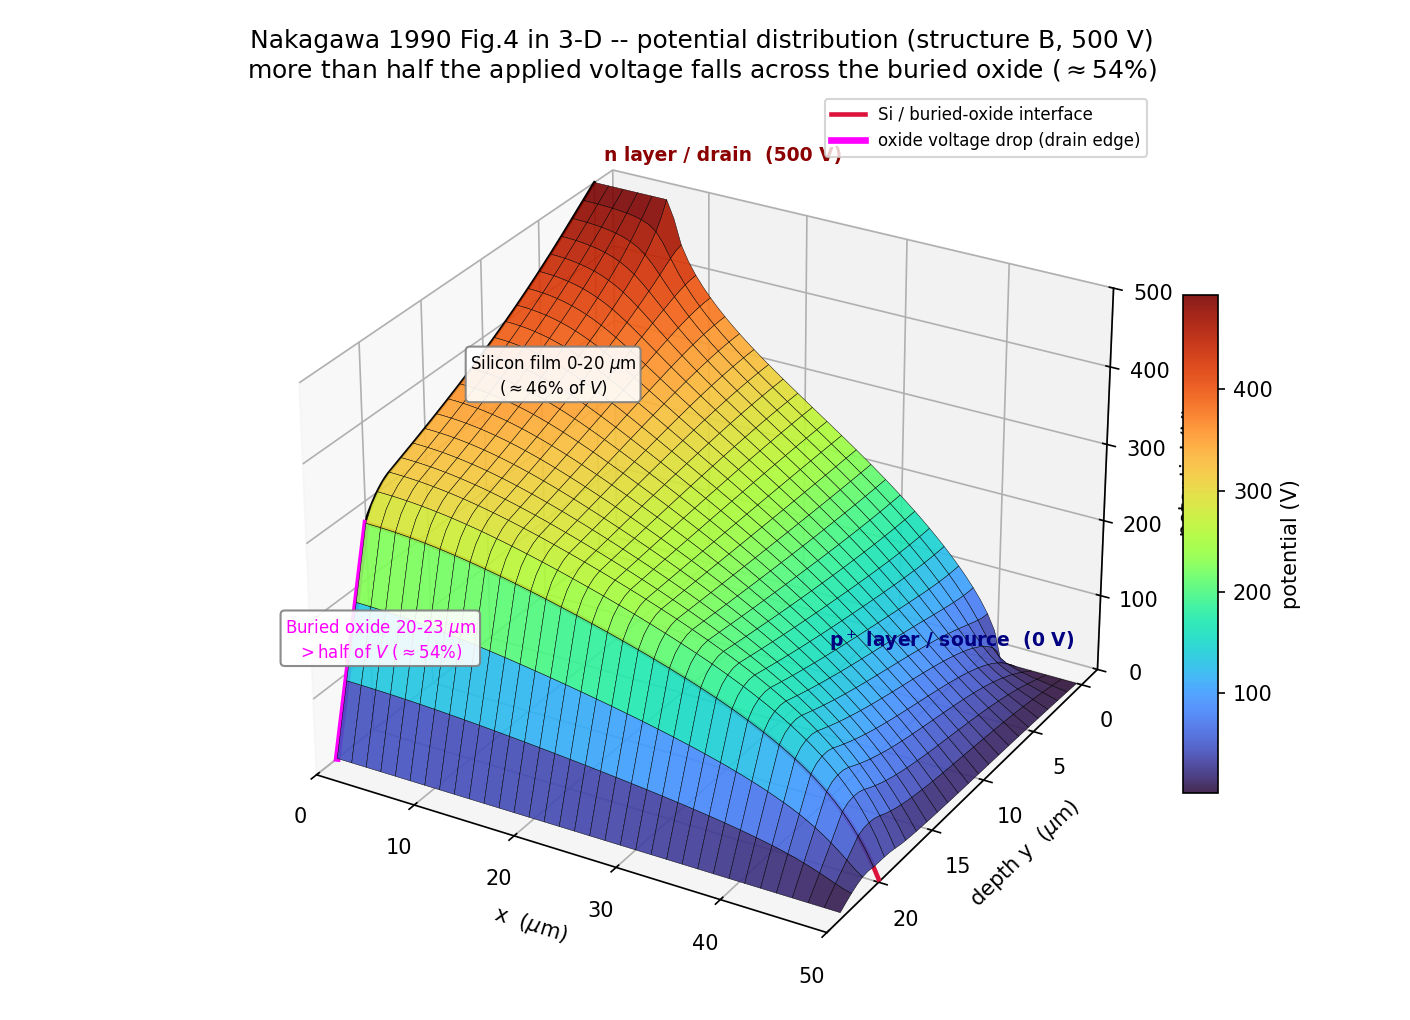
\includegraphics[width=\linewidth]{../figs/fig4_potential_3d.png}
\caption{This reproduction (3-D)}
\end{subfigure}
\\[6pt]
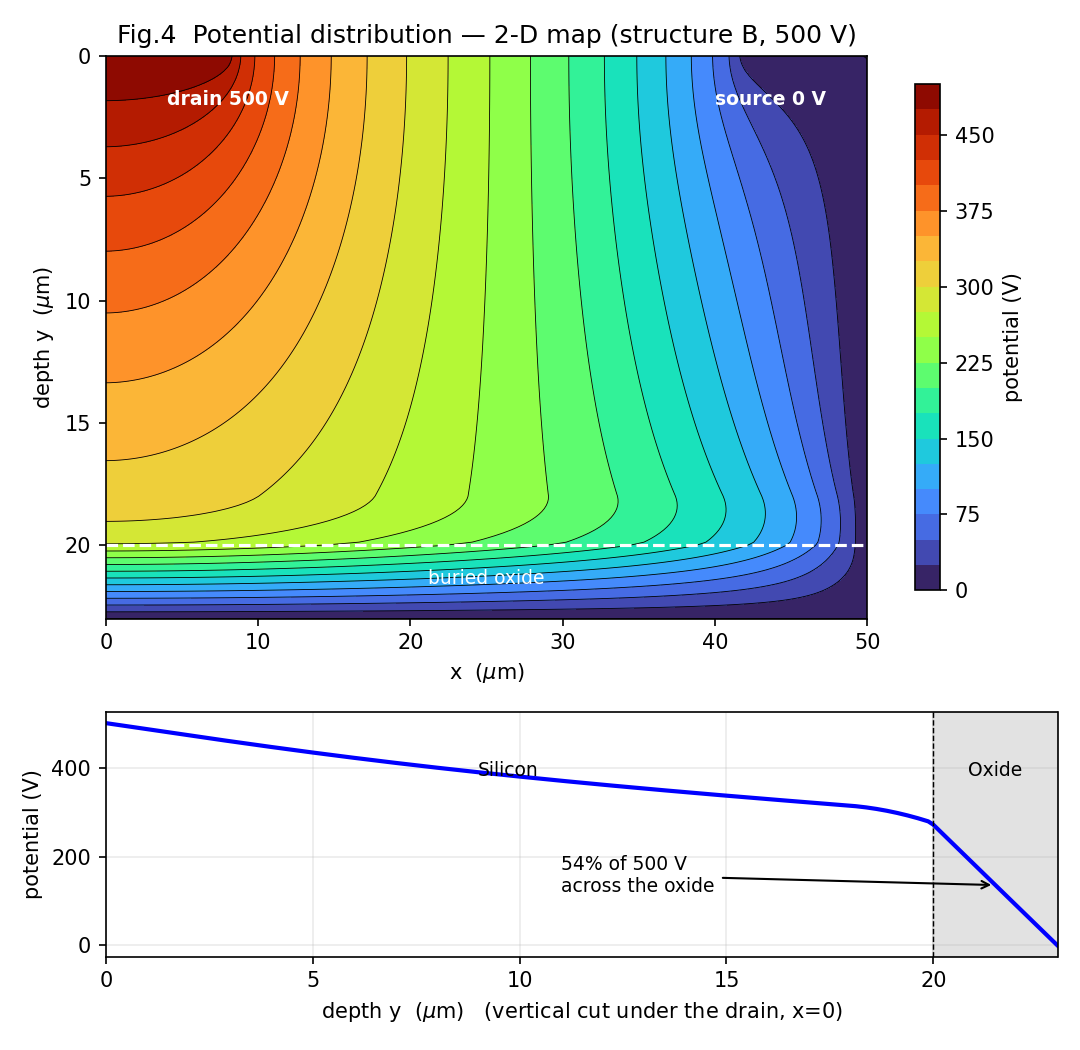
\includegraphics[width=0.72\textwidth]{../figs/fig4_potential.png}
\caption{\textbf{Fig.~4 --- potential distribution (structure~B, \SI{500}{\volt}).}
Both show a \SI{500}{\volt} plateau at the $n$-layer/drain sloping to the $p^+$
side, with a steep face over the oxide film --- the $>$half-voltage drop across
the buried oxide. The 2-D map (bottom) quantifies it: 54\,\% of \SI{500}{\volt}
falls across the oxide under the drain.}
\end{figure}

\begin{figure}[h!]
\centering
\begin{subfigure}{0.46\textwidth}
\includegraphics[width=\linewidth]{../figs_paper/fig5_paper_crop.png}
\caption{Paper (original)}
\end{subfigure}\hfill
\begin{subfigure}{0.52\textwidth}
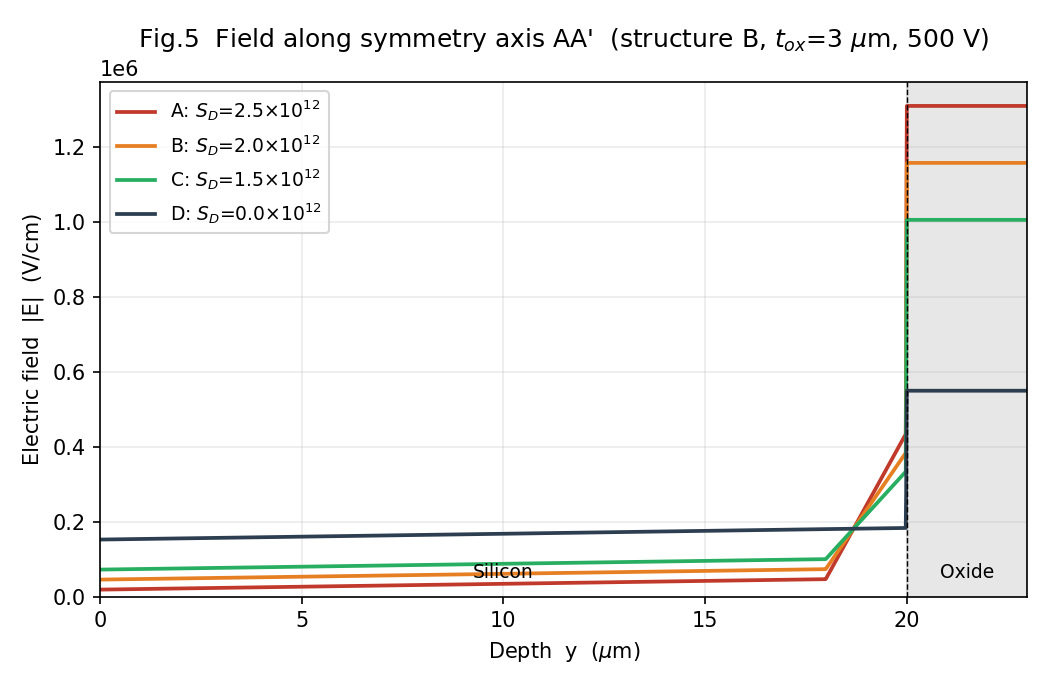
\includegraphics[width=\linewidth]{../figs/fig5_field.png}
\caption{This reproduction}
\end{subfigure}
\caption{\textbf{Fig.~5 --- electric field along the symmetry axis $AA'$}
($\tox=\SI{3}{\micro\meter}$, \SI{500}{\volt}). In the silicon the field is low
and ordered $D>C>B>A$ (more dose $\Rightarrow$ more shielding); it jumps $\sim\!3\times$
at the Si/oxide interface and is constant across the charge-free oxide. The paper's
oxide bars (A highest, D lowest) match the model's oxide field.}
\end{figure}

\begin{figure}[h!]
\centering
\begin{subfigure}{0.46\textwidth}
\includegraphics[width=\linewidth]{../figs_paper/fig6_paper_crop.png}
\caption{Paper (original)}
\end{subfigure}\hfill
\begin{subfigure}{0.52\textwidth}
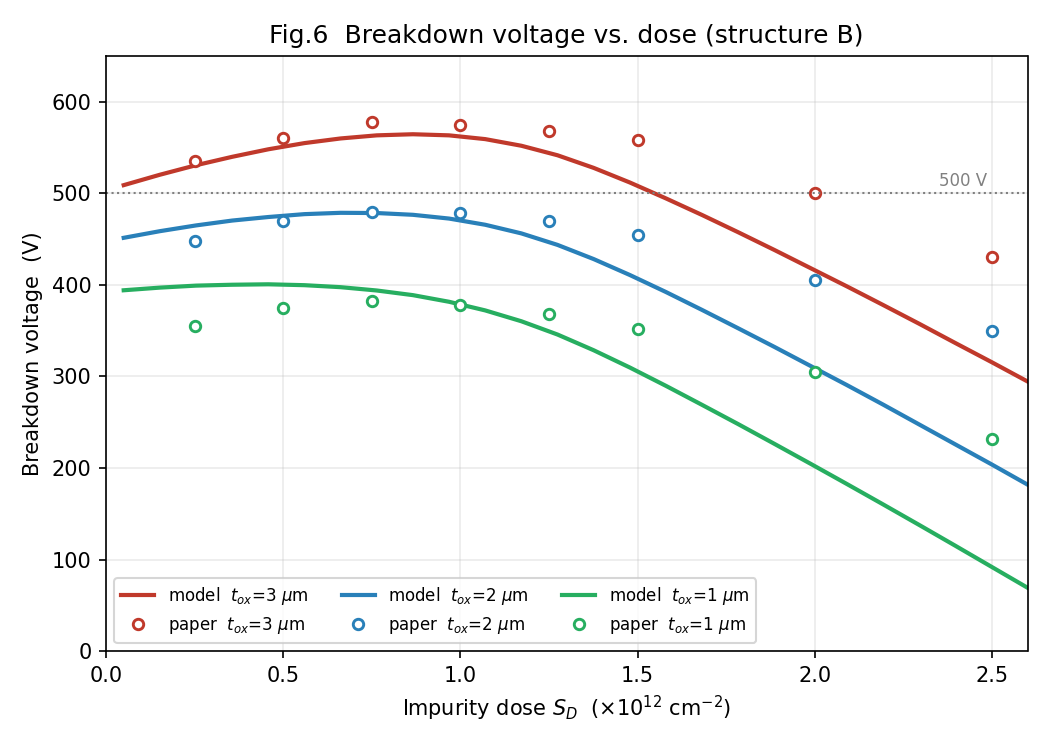
\includegraphics[width=\linewidth]{../figs/fig6_bv.png}
\caption{This reproduction}
\end{subfigure}
\caption{\textbf{Fig.~6 --- breakdown voltage vs.\ dose (structure~B).}
Model curves (lines) vs.\ digitized paper points (circles) for
$\tox=1,2,3\ \si{\micro\meter}$. The RESURF optimum --- $BV$ rising with dose,
peaking near $\SI{1e12}{\per\square\centi\meter}$, then falling --- is reproduced,
with peak $BV\sim400/480/565\ \si{\volt}$ vs.\ the paper's
$\sim\!380/480/580\ \si{\volt}$.}
\end{figure}

\begin{figure}[h!]
\centering
\begin{subfigure}{0.40\textwidth}
\includegraphics[width=\linewidth]{../figs_paper/fig7_paper_crop.png}
\caption{Paper (original)}
\end{subfigure}\hfill
\begin{subfigure}{0.56\textwidth}
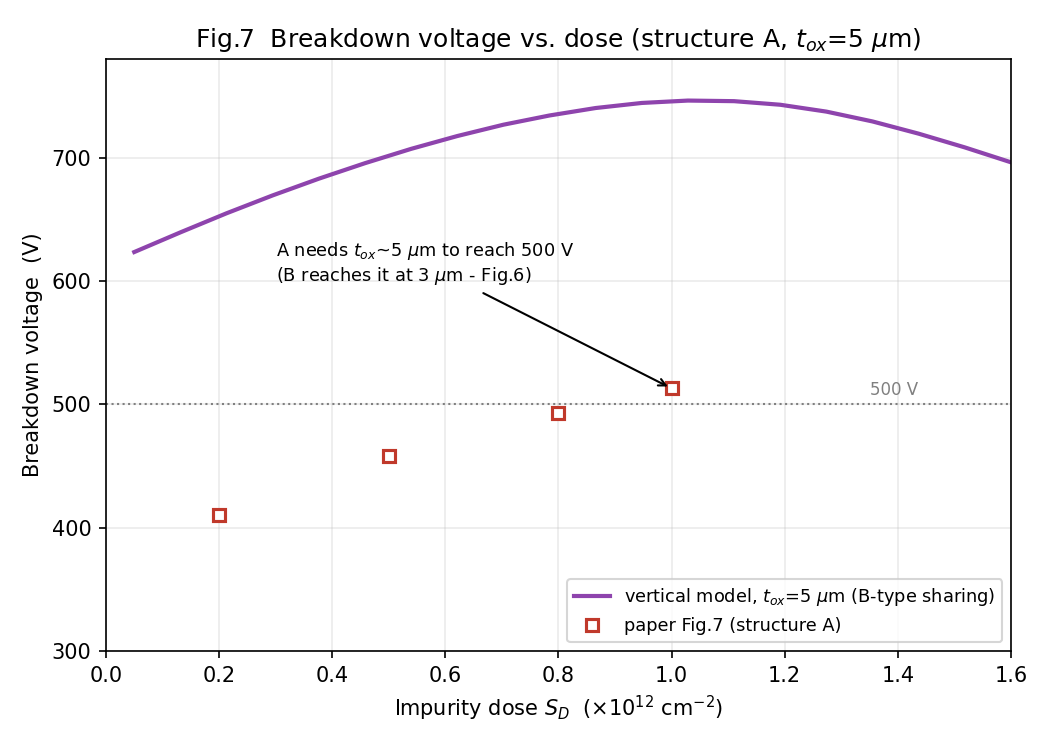
\includegraphics[width=\linewidth]{../figs/fig7_bv.png}
\caption{This reproduction}
\end{subfigure}
\caption{\textbf{Fig.~7 --- breakdown voltage vs.\ dose (structure~A,
$\tox=\SI{5}{\micro\meter}$).} The vertical model (purple, B-type sharing) lies
above the structure-A data because A and B share the same vertical stack --- their
difference is 2-D. The gap ($\sim$150--200\,V) is the signature of A's less
complete field-sharing, consistent with A needing \SI{5}{\micro\meter} oxide where
B needs \SI{3}{\micro\meter}.}
\end{figure}

\clearpage
\section{Notes and limitations}
\textbf{What matches:} the oxide carries $>$half the voltage (Fig.~4, model
54--60\,\%); the field shielding by the donor sheet (Fig.~5) with the correct
ordering and $\sim\!3\times$ interface jump; the $BV(\SD)$ RESURF curves and
magnitudes (Fig.~6) within $\sim\!5\,\%$.\\[4pt]
\textbf{Known limitation:} structure~A (Fig.~7) is a 2-D effect; the vertical model
over-predicts its absolute $BV$. Reproducing it quantitatively requires the full
2-D device with the actual asymmetric drain/sinker doping.\\[4pt]
\textbf{Code:} \texttt{nakagawa1990\_full.py} (single-file PDE~$\to$~plots),
\texttt{model.py} (1-D electrostatics + avalanche), \texttt{solver2d.py} (2-D
Poisson), \texttt{fig4--fig7\_*.py} (figure scripts), \texttt{derivation.md} (full
analytic derivation).

\end{document}
